\chapter{Results}\label{ch:results}
In this chapter, we present the results of our experiments.

\section{Clone types}\label{sec:clonetypeexperiments}
In this section we display the differences between clone type 1-3~\cite{roy2007survey} and type 1R-3R as proposed in chapter \ref{chap:clonetypes}. When running our clone detection script over the corpus, we get the results displayed in Fig.~\ref{fig:typeres}.

\begin{figure}[H]
  \caption{Number of cloned declarations/statements.}
    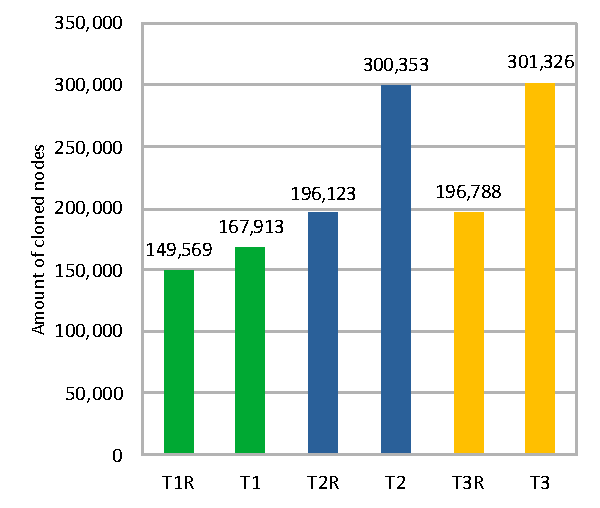
\includegraphics[width=.5\columnwidth]{img/TypeResults}
  \label{fig:typeres}
\end{figure}

In this figure, the number of cloned nodes per clone type are displayed. The difference between T1R and T1 is small (10.9\%), because most often textually equal code is also functionally equal. The difference between T2R and T2 is bigger (34.7\%) because the T2R definition is more strict. T3R and T3 are similar to T2R and T2 because our dataset does not have so many gapped clones for the thresholds used.

We also measured the duration of finding clones by the different clone types. Fig.~\ref{fig:performance} shows the duration of detecting all clones in the corpus using CloneRefactor for different clone types. Although this data is partly dependent on our implementation of the clone types, there is a notable difference between the refactoring-oriented clone types and the literature clone types. The reason for this is further explained in Sec.~\ref{chap:challenge}.

\begin{figure}[H]
  \caption{Duration in minutes of identifying clones for clone type definitions.}
    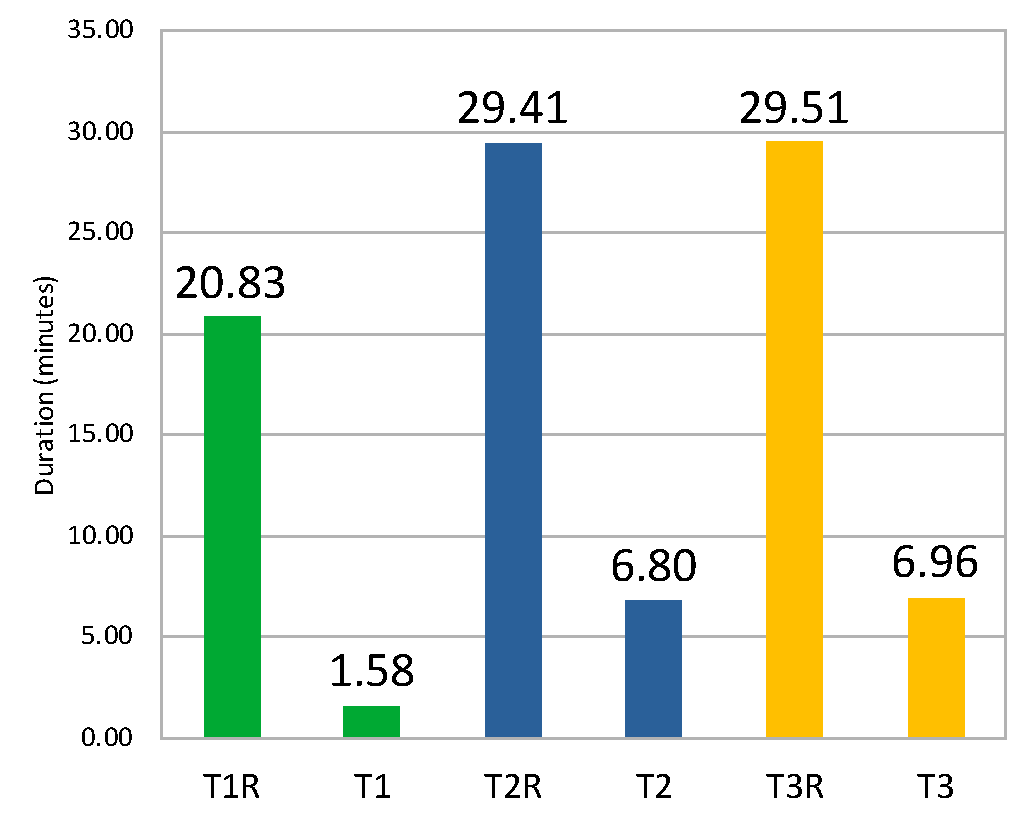
\includegraphics[width=.5\columnwidth]{img/DurationChart}
  \label{fig:performance}
\end{figure}

\section{Thresholds} \label{sec:thresholds}
\todo{todo}

\section{Context Analysis of Clones}\label{chap:clonecontextexpl}
We analyzed the context of clones in a large corpus of open source projects. For these experiments, we used our CloneRefactor tool. These experiments follow the structure of the context: The relation between clone instances is explained, measured and discussed in chapter \ref{chap:relationsinstances}; the location of clone instances is explained, measured and discussed in chapter \ref{chap:clonelocation};  the content of clone instances are explained, measured and discussed in chapter \ref{chap:clonecontents}.

\subsection{Clone detection results}
Currently, we have implemented two clone detection algorithms into CloneRefactor. The first one finds clones by comparing tokens (excluding whitespace, comments and newlines), equal to the definition of type 1 clones in literature \cite{roy2007survey}. The second algorithm implements our type 1R, as explained in chapter \ref{chap:type1clones}. The differences between the clones found for these algorithms is displayed in Table \ref{table:clonedet}.

\begin{table}[H]
  \begin{center}
  \caption{CloneRefactor clone detection results for the two different algorithms.} \label{table:clonedet}
  \medskip
\begin{tabular}{|l|l|l|}
\hline
 & \textbf{Type 1} & \textbf{Type 1R} \\ \hline
\begin{tabular}[c]{@{}l@{}}Amount of lines cloned\end{tabular} & 200,362 & 129,519 \\ \hline
\begin{tabular}[c]{@{}l@{}}Amount of statements/\\declarations cloned\end{tabular} & 182,466 & 118,980 \\ \hline
\begin{tabular}[c]{@{}l@{}}Amount of tokens cloned\end{tabular} & 1,582,845 & 973,596 \\ \hline
\end{tabular}
\end{center}
\end{table}

Looking at Table \ref{table:clonedet}, it becomes apparent that the type 1R algorithm finds significantly less clones than the type 1 algorithm. This indicates that about a third of the clones have textual equality, but are not actually equal when considering the types of expressions. This makes these clones less suitable for automated refactoring.

\subsection{Relations Between Clone Instances} \label{chap:relationsinstances}
In section \ref{sec:setuprelation} we introduced our experiments regarding relations between clones. Table~\ref{table:relations} contains our results regarding the relations between clone instances.

\begin{table}[H]
  \begin{center}
  \caption{Clone relations} \label{table:relations}
  \medskip
\begin{tabular}{|l|l|l|} \hline
\textbf{Relation} & \textbf{\#} & \textbf{\%} \\ \hline
Unrelated          & 12,368 & 34.88            \\ \hline
Same Class          & 11,483 & 32.38             \\ \hline
Same Method               & 5,056 & 14.26            \\ \hline
Sibling         & 4,182 & 11.79             \\ \hline
External Superclass   & 1,066 & 3.01             \\ \hline
Superclass          & 558 & 1.57           \\ \hline
First Cousin          & 489 & 1.38           \\ \hline
Common Hierarchy    & 206 & 0.58            \\ \hline
Ancestor          & 54 & 0.15          \\ \hline
\end{tabular}
\end{center}
\end{table}

The most notable difference when comparing it to the results of Fontana et al.~\cite{fontana2015duplicated} is that in our results most of the clones are unrelated (34.44\%), while for them it was only 15.70\%. This is likely due to the fact that we consider clone classes rather than clone pairs, and mark the clone class ``Unrelated'' even if just one of the clone instances is outside a hierarchy. It could also be that the corpus which we use, as it has generally smaller projects, uses more classes from outside the project (which are marked ``Unrelated'' if they do not have a common external superclass). About a third of all clone classes have all instances in the same class, which is generally easy to refactor. On the third place come the clones that are in the same method, which are similarly easy to refactor.

\subsection{Clone instance location}\label{chap:clonelocation}
Measuring the clone locations categories defined in section \ref{sec:setuplocation} yields the results displayed in Table \ref{table:contents}.

\begin{table}[H]
  \begin{center}
  \caption{Clone instance locations} \label{table:locations}
  \medskip
\begin{tabular}{|l|l|l|}
\hline
\textbf{Location}   & \textbf{\#} & \textbf{\%} \\ \hline
Method Level        & 83,813 & 82.62            \\ \hline
Class Level        & 12,534 & 12.35            \\ \hline
Constructor Level    & 4,391 & 4.33           \\ \hline
Interface Level   & 567 & 0.56           \\ \hline
Enum Level         & 145 & 0.14            \\ \hline
\end{tabular}
\end{center}
\end{table}

Our results indicate that around 58\% of the clones are produced at method-level. About 39\% of clones either span several methods/constructors or contain something like a field declaration. Another 3\% of the clones are found in constructors. The amount of clones found in interfaces and enumerations is very low. Regarding the differences between type 1 and type 1R, it seems that there are relatively less method level clones and more class level clones for type 1R. This is probably due to that the main reason for variability between type 1 and type 1R is variable references, which occur more at method level than class level.

\section{Clone instance contents}\label{chap:clonecontents}
Measuring the clone contents categories defined in section \ref{sec:setupcontents} yields the results displayed in Table \ref{table:contents}.

\begin{table}[H]
  \begin{center}
  \caption{Clone instance contents} \label{table:contents}
  \medskip
\begin{tabular}{|l|l|l|}
  \hline
  \textbf{Contents} & \textbf{\#} & \textbf{\%} \\ \hline
  Partial Method     & 79,945 & 78.80 \\ \hline
  Several Methods         & 7,323 & 7.22 \\ \hline
  Partial Constructor      & 4,385 & 4.32 \\ \hline
  Full Method           & 3,868 & 3.81 \\ \hline
  Only Fields           & 3,039 & 3.00 \\ \hline
  Includes Constructor  & 1,522 & 1.50 \\ \hline
  Includes Field        & 616 & 0.61 \\ \hline
  Includes Class Declaration  & 376 & 0.37 \\ \hline
  Other Categories    & 376 & 0.37\\ \hline
\end{tabular}
\end{center}
\end{table}

Unsurprisingly, most clones span a part of a method. The most used refactoring technique for clones that span part of a method is ``Extract Method''. Because of that, we focus our research efforts on refactoring such clones.

\section{Merging duplicate code through refactoring} \label{sec:refactorability}
In section \ref{sec:refactorabilitysetup} we define catagories regarding the extent to which clones can be refactored through method extraction. Our results are displayed in Table \ref{table:refactorability}.

\begin{table}[H]
  \begin{center}
  \caption{Refactorability through method extraction} \label{table:refactorability}
  \medskip
\begin{tabular}{|l|l|l|}
\hline
\textbf{}         & \textbf{\#} & \textbf{\%} \\ \hline
Can be extracted     & 14,664 & 41.35 \\ \hline
Spans part of a block  & 10,801 & 30.46 \\ \hline
Is not a partial method   & 8,074 & 22.77 \\ \hline
Complex control flow & 1,922 & 5.42 \\ \hline
\end{tabular}
\end{center}
\end{table}

From Table~\ref{table:refactorability}, we can see that 41\% of the clones can directly be refactored through method extraction (and possibly other refactoring techniques based on the relation of the clone instances). For the other clones, other techniques or transformations will be required.

\section{Refactoring clones}
\todo{TODO}
